\section{Results}

Tests were conducted on an Inspiron 15 7000, with 3 parties
running locally in an Ubuntu 16.04 virtual machine.
The fact that the programs ran on a single machine impacts
the running time of the program, (since there is no latency,
but at the same time there is increased compuation demand).
We therefore only report on total communication cost
since this should be approximately uniform accross testing
environments. 
\footnote{Running programs on a single machine means there
is no packet loss. Therefore it can be expected to have
slightly improved communication cost relative to running
the protocol in a real network, but this affect should be small.}

SCALE-MAMBA prepares pre-processing data in batches.
Therefore, if a program is small, and does not use 
an entire batch, it will have much higher communication cost
than if it were run as part of a larger computation.
To compensate for this, we ran smaller tests multiple times and 
found the average cost per execution.

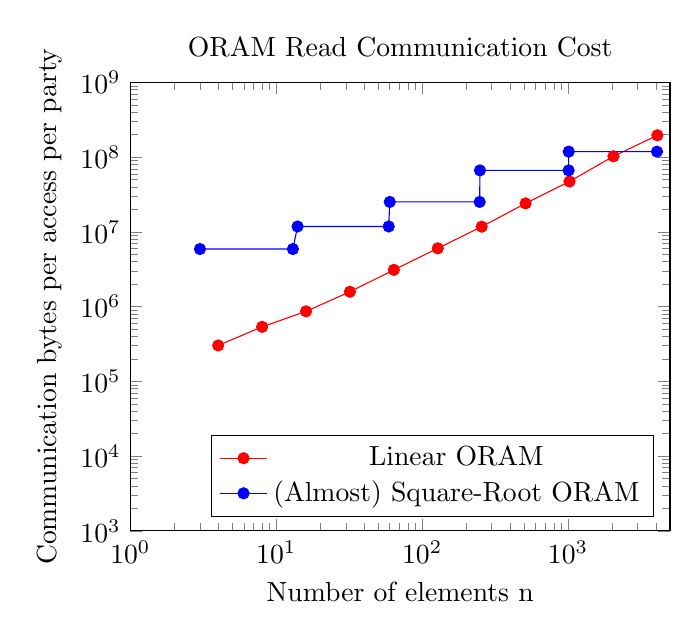
\begin{tikzpicture}
\begin{axis}[
title={ORAM Read Communication Cost},
xlabel={Number of elements n},
ylabel={Communication bytes per access per party},
xmin=1, xmax=5000,
ymin=1000, ymax=1000000000,
legend pos=south east,
xmode=log,
ymode=log,
]

\addplot[
  color=red,
  mark=*
]
coordinates{
(4, 302424) (8, 536528) (16, 865603) (32, 1582736) (64, 3108361)
(128, 6028379) (256, 11754377) (512, 24092308) (1024, 47349607)
(2048, 102830129) (4096, 196480184)
};

\addplot[
  color=blue,
  mark=*
]
coordinates{
(3, 5904926) (13, 5904926) (14, 11831676) (59, 11831676)
(60, 25207763) (248, 25207763) (249, 66609406)
(1010, 66609406) (1011, 118715054) (4073, 118715054)
};
\legend{Linear ORAM, (Almost) Square-Root ORAM}

\end{axis}
\end{tikzpicture}
